\documentclass[]{article}
\usepackage{lmodern}
\usepackage{amssymb,amsmath}
\usepackage{ifxetex,ifluatex}
\usepackage{fixltx2e} % provides \textsubscript
\ifnum 0\ifxetex 1\fi\ifluatex 1\fi=0 % if pdftex
  \usepackage[T1]{fontenc}
  \usepackage[utf8]{inputenc}
\else % if luatex or xelatex
  \ifxetex
    \usepackage{mathspec}
  \else
    \usepackage{fontspec}
  \fi
  \defaultfontfeatures{Ligatures=TeX,Scale=MatchLowercase}
  \newcommand{\euro}{€}
\fi
% use upquote if available, for straight quotes in verbatim environments
\IfFileExists{upquote.sty}{\usepackage{upquote}}{}
% use microtype if available
\IfFileExists{microtype.sty}{%
\usepackage{microtype}
\UseMicrotypeSet[protrusion]{basicmath} % disable protrusion for tt fonts
}{}
\usepackage[margin=1in]{geometry}
\usepackage{hyperref}
\PassOptionsToPackage{usenames,dvipsnames}{color} % color is loaded by hyperref
\hypersetup{unicode=true,
            pdftitle={Predicting Total Wins Per Season in Major Leauge Baseball from Game Statistics},
            pdfauthor={Daniel Brooks (daniel.brooks@spsmail.cuny.edu), Daniel Fanelli (daniel.fanelli@spsmail.cuny.edu), Christopher Fenton (christopher.fenton@spsmail.cuny.edu), James Hamski (james.hamski@spsmail.cuny.edu), Youqing Xiang (youqing.xiang@spsmail.cuny.edu)},
            pdfborder={0 0 0},
            breaklinks=true}
\urlstyle{same}  % don't use monospace font for urls
\usepackage{color}
\usepackage{fancyvrb}
\newcommand{\VerbBar}{|}
\newcommand{\VERB}{\Verb[commandchars=\\\{\}]}
\DefineVerbatimEnvironment{Highlighting}{Verbatim}{commandchars=\\\{\}}
% Add ',fontsize=\small' for more characters per line
\usepackage{framed}
\definecolor{shadecolor}{RGB}{248,248,248}
\newenvironment{Shaded}{\begin{snugshade}}{\end{snugshade}}
\newcommand{\KeywordTok}[1]{\textcolor[rgb]{0.13,0.29,0.53}{\textbf{{#1}}}}
\newcommand{\DataTypeTok}[1]{\textcolor[rgb]{0.13,0.29,0.53}{{#1}}}
\newcommand{\DecValTok}[1]{\textcolor[rgb]{0.00,0.00,0.81}{{#1}}}
\newcommand{\BaseNTok}[1]{\textcolor[rgb]{0.00,0.00,0.81}{{#1}}}
\newcommand{\FloatTok}[1]{\textcolor[rgb]{0.00,0.00,0.81}{{#1}}}
\newcommand{\ConstantTok}[1]{\textcolor[rgb]{0.00,0.00,0.00}{{#1}}}
\newcommand{\CharTok}[1]{\textcolor[rgb]{0.31,0.60,0.02}{{#1}}}
\newcommand{\SpecialCharTok}[1]{\textcolor[rgb]{0.00,0.00,0.00}{{#1}}}
\newcommand{\StringTok}[1]{\textcolor[rgb]{0.31,0.60,0.02}{{#1}}}
\newcommand{\VerbatimStringTok}[1]{\textcolor[rgb]{0.31,0.60,0.02}{{#1}}}
\newcommand{\SpecialStringTok}[1]{\textcolor[rgb]{0.31,0.60,0.02}{{#1}}}
\newcommand{\ImportTok}[1]{{#1}}
\newcommand{\CommentTok}[1]{\textcolor[rgb]{0.56,0.35,0.01}{\textit{{#1}}}}
\newcommand{\DocumentationTok}[1]{\textcolor[rgb]{0.56,0.35,0.01}{\textbf{\textit{{#1}}}}}
\newcommand{\AnnotationTok}[1]{\textcolor[rgb]{0.56,0.35,0.01}{\textbf{\textit{{#1}}}}}
\newcommand{\CommentVarTok}[1]{\textcolor[rgb]{0.56,0.35,0.01}{\textbf{\textit{{#1}}}}}
\newcommand{\OtherTok}[1]{\textcolor[rgb]{0.56,0.35,0.01}{{#1}}}
\newcommand{\FunctionTok}[1]{\textcolor[rgb]{0.00,0.00,0.00}{{#1}}}
\newcommand{\VariableTok}[1]{\textcolor[rgb]{0.00,0.00,0.00}{{#1}}}
\newcommand{\ControlFlowTok}[1]{\textcolor[rgb]{0.13,0.29,0.53}{\textbf{{#1}}}}
\newcommand{\OperatorTok}[1]{\textcolor[rgb]{0.81,0.36,0.00}{\textbf{{#1}}}}
\newcommand{\BuiltInTok}[1]{{#1}}
\newcommand{\ExtensionTok}[1]{{#1}}
\newcommand{\PreprocessorTok}[1]{\textcolor[rgb]{0.56,0.35,0.01}{\textit{{#1}}}}
\newcommand{\AttributeTok}[1]{\textcolor[rgb]{0.77,0.63,0.00}{{#1}}}
\newcommand{\RegionMarkerTok}[1]{{#1}}
\newcommand{\InformationTok}[1]{\textcolor[rgb]{0.56,0.35,0.01}{\textbf{\textit{{#1}}}}}
\newcommand{\WarningTok}[1]{\textcolor[rgb]{0.56,0.35,0.01}{\textbf{\textit{{#1}}}}}
\newcommand{\AlertTok}[1]{\textcolor[rgb]{0.94,0.16,0.16}{{#1}}}
\newcommand{\ErrorTok}[1]{\textcolor[rgb]{0.64,0.00,0.00}{\textbf{{#1}}}}
\newcommand{\NormalTok}[1]{{#1}}
\usepackage{longtable,booktabs}
\usepackage{graphicx,grffile}
\makeatletter
\def\maxwidth{\ifdim\Gin@nat@width>\linewidth\linewidth\else\Gin@nat@width\fi}
\def\maxheight{\ifdim\Gin@nat@height>\textheight\textheight\else\Gin@nat@height\fi}
\makeatother
% Scale images if necessary, so that they will not overflow the page
% margins by default, and it is still possible to overwrite the defaults
% using explicit options in \includegraphics[width, height, ...]{}
\setkeys{Gin}{width=\maxwidth,height=\maxheight,keepaspectratio}
\setlength{\parindent}{0pt}
\setlength{\parskip}{6pt plus 2pt minus 1pt}
\setlength{\emergencystretch}{3em}  % prevent overfull lines
\providecommand{\tightlist}{%
  \setlength{\itemsep}{0pt}\setlength{\parskip}{0pt}}
\setcounter{secnumdepth}{5}

%%% Use protect on footnotes to avoid problems with footnotes in titles
\let\rmarkdownfootnote\footnote%
\def\footnote{\protect\rmarkdownfootnote}

%%% Change title format to be more compact
\usepackage{titling}

% Create subtitle command for use in maketitle
\newcommand{\subtitle}[1]{
  \posttitle{
    \begin{center}\large#1\end{center}
    }
}

\setlength{\droptitle}{-2em}
  \title{Predicting Total Wins Per Season in Major Leauge Baseball from Game
Statistics}
  \pretitle{\vspace{\droptitle}\centering\huge}
  \posttitle{\par}
  \author{Daniel Brooks
(\href{mailto:daniel.brooks@spsmail.cuny.edu}{\nolinkurl{daniel.brooks@spsmail.cuny.edu}}),
Daniel Fanelli
(\href{mailto:daniel.fanelli@spsmail.cuny.edu}{\nolinkurl{daniel.fanelli@spsmail.cuny.edu}}),
Christopher Fenton
(\href{mailto:christopher.fenton@spsmail.cuny.edu}{\nolinkurl{christopher.fenton@spsmail.cuny.edu}}),
James Hamski
(\href{mailto:james.hamski@spsmail.cuny.edu}{\nolinkurl{james.hamski@spsmail.cuny.edu}}),
Youqing Xiang
(\href{mailto:youqing.xiang@spsmail.cuny.edu}{\nolinkurl{youqing.xiang@spsmail.cuny.edu}})}
  \preauthor{\centering\large\emph}
  \postauthor{\par}
  \predate{\centering\large\emph}
  \postdate{\par}
  \date{6/19/2016}



% Redefines (sub)paragraphs to behave more like sections
\ifx\paragraph\undefined\else
\let\oldparagraph\paragraph
\renewcommand{\paragraph}[1]{\oldparagraph{#1}\mbox{}}
\fi
\ifx\subparagraph\undefined\else
\let\oldsubparagraph\subparagraph
\renewcommand{\subparagraph}[1]{\oldsubparagraph{#1}\mbox{}}
\fi

\begin{document}
\maketitle

\section{Introduction}\label{introduction}

Baseballl is a sport that follows a sequence of pitches, at-bats, and
innings where play is contained between discrete pitches. Unlike the
more continuous play of soccer or basketball, this makes baseball
conducive to gathering extensive data on individual and team
performance.

In this report we attempt to model wins per season for Major League
Baseball (MLB) teams (response variable). Our dataset includes 15
potential predictor variables, adjusted to reflect a standardized 162
game season, using MLB records from 1871 to 2006.

\section{Data Exploration}\label{data-exploration}

\subsection{Response Variable}\label{response-variable}

Team Wins (TARGET\_WINS) appears to be normally distributed with a
slight left skew and a mean of 80.79, which is half of the total 162
game season.\\
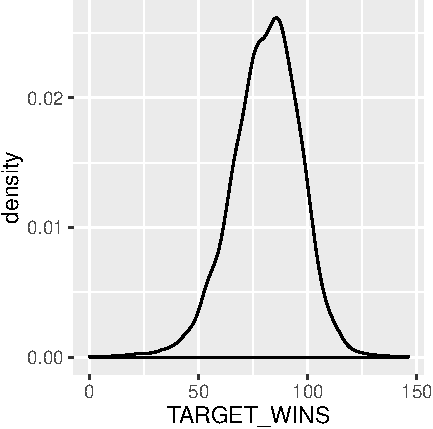
\includegraphics{DATA621-Homework-1_files/figure-latex/unnamed-chunk-3-1.pdf}

\subsection{Predictor Variables}\label{predictor-variables}

Most of the predictor variables appear to be approximately normally
distributed. Interesesting results include:

Homeruns (TEAM\_BATTING\_HR) appears to be multinomial. Because the
dataset contains game results from 1871 to 2006, it includes time
periods which are known to have influenced the occurance of homeruns,
including ``The Steriod Era'' and the introduction of the designated
hitter in the American League
\href{https://www.washingtonpost.com/news/fancy-stats/wp/2016/03/07/the-perfect-storm-that-created-baseballs-biggest-home-run-surge-since-the-steroid-era/}{Greenberg,
N. 2016}. Batting Strikeouts (TEAM\_BATTING\_STRIKEOUTS) also appears
multinomial.

\emph{Histograms indicating the distribution of each variable}\\
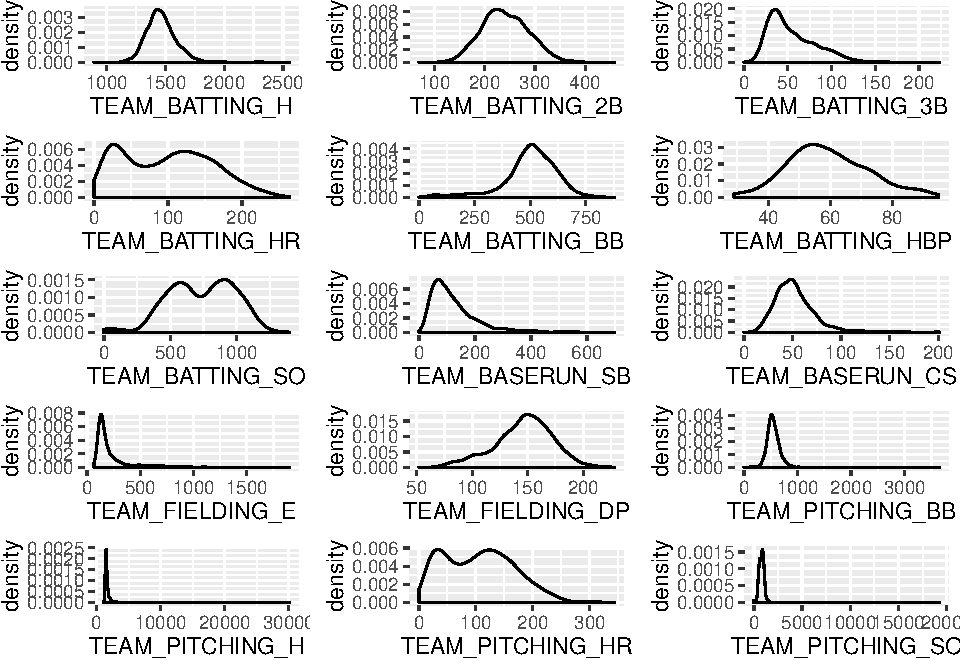
\includegraphics{DATA621-Homework-1_files/figure-latex/unnamed-chunk-4-1.pdf}

The only variables which appear to be positively correlated with Team
Wins over their entire range are Hits by Batters (TEAM\_BATTING\_H) and
Doubles by Batters (TEAM\_BATTING\_2B). Errors (TEAM\_FIELDING\_E) is
negatively correlated with wins at it's larger values. For the rest of
the predictor variables, a smoothed conditional mean indicates a trend
when plotted against Team Wins only at extreme high or low values where
data points are sparse, or no trend at all.

\emph{Predictor variables plotted versus Team Wins, including a smoothed
conditional mean}\\
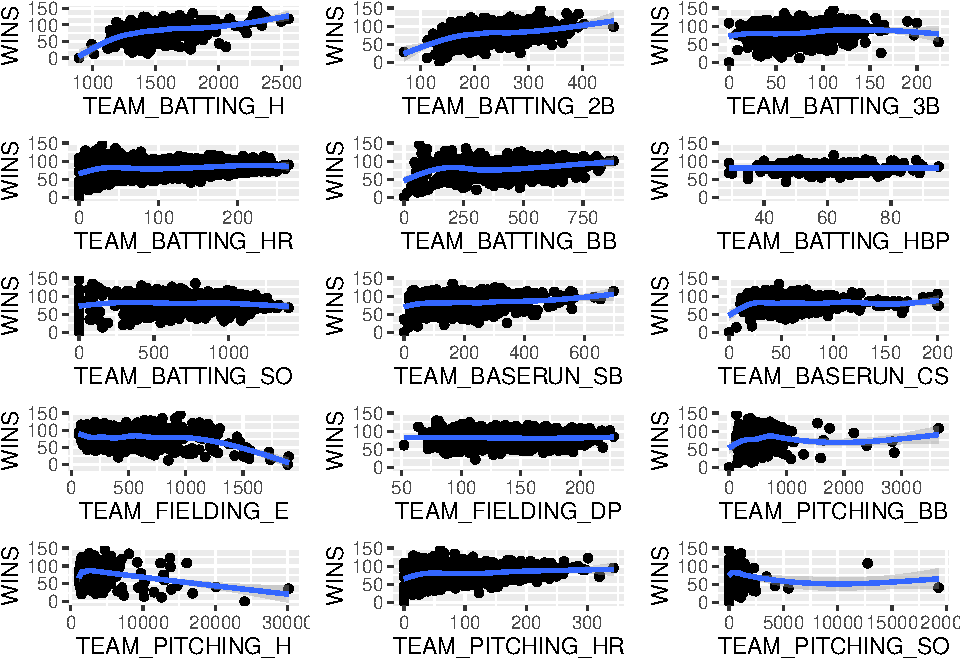
\includegraphics{DATA621-Homework-1_files/figure-latex/unnamed-chunk-5-1.pdf}

\section{Data Preparation}\label{data-preparation}

\subsection{Outliers and Non-sensical
Values}\label{outliers-and-non-sensical-values}

The histograms and scatterplots above indicate a few variables which
have outliers or non-sensical values.

\paragraph{Base Hits by Batters, Doubles, Triples,
Homeruns}\label{base-hits-by-batters-doubles-triples-homeruns}

No changes made.

\paragraph{Strikeouts by Batters}\label{strikeouts-by-batters}

Several 0 values were replaced with NAs, as it is virtually impossible
to make it through an entire season with zero strike outs. The next low
value (66) indicates 0 is missing data in this variable.

\paragraph{Hit by Pitch}\label{hit-by-pitch}

See \textbf{Missing Data} section below.

\paragraph{Strikeout by Batters, Stolen bases, Caught Stealing, Errors,
Double
Plays}\label{strikeout-by-batters-stolen-bases-caught-stealing-errors-double-plays}

No changes made.

\paragraph{Errors, Walks Allowed, Strikeouts by
Pitchers}\label{errors-walks-allowed-strikeouts-by-pitchers}

Two outlier values for TEAM\_PITCHING\_SO are higher than the total
number of out during a season excluding extra innings (4,374). In
addition, these series tended to have unreasonably long right skewed
tails. Therefore, high outliers, as defnited by three standard
deviations from the mean, were replaced with NAs.

\paragraph{Hits Allowed}\label{hits-allowed}

We would expect the maximum Hits Allowed (TEAM\_PITCHING\_H) to be on
par with the maximum Hits by Batters (TEAM\_BATTING\_H). However, Hits
allowed has many values that are thousands higher than Hits by Batters.
Therefore, Hits Allowed greater than the maximum Hits by Batters were
replaced with NAs.

\subsection{Multicollinearity}\label{multicollinearity}

One of the challenges of this dataset is the existence of variables that
are by-definition correlated. For a complete dataset for the variables
here, for all teams in MLB, several variables will have common sums. Dy
definition: for every one Hit by Batters there will be one Hit Allowed.
This is the case for: Hits (singles through homeruns), strikeouts and
walks. Teams tend to play within their leauge (American Leauge /
National Leauge) and within their division frequently. This is perhaps
an explanation for the existence of collinearity in the dataset.

In addition, some variables are indicators of frequency attempted.
Caught stealing and stolen bases are highly correlated by team. They're
also correlated by individual player - Ricky Henderson holds the MLB
record for stolen bases at 1,406 - but he also holds the record for most
times caught stealing, at 335.
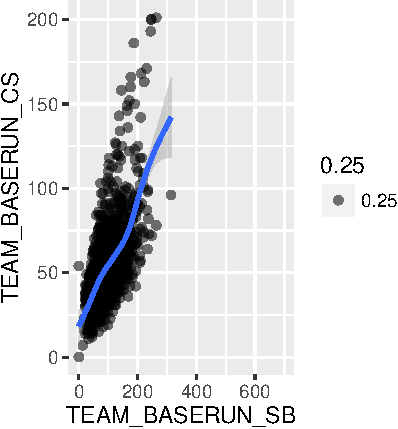
\includegraphics{DATA621-Homework-1_files/figure-latex/unnamed-chunk-10-1.pdf}

\emph{Correlation plot for the indicator and all predictor variables}\\
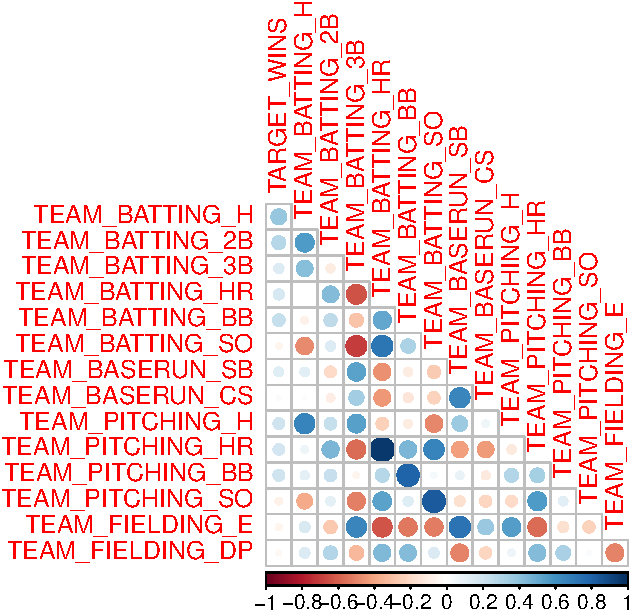
\includegraphics{DATA621-Homework-1_files/figure-latex/unnamed-chunk-11-1.pdf}

\subsection{Missing Data}\label{missing-data}

In statistical analysis, it is important remain mindful of context and
not ignore the mechanics of the system being studied. Hit-by-Pitch is
missing 2085 records - 90\% of the dataset. This variable was dropped
completely from the dataset and ignored by future analysis for two
reasons (1) the vast majority of records were missing and (2)
hit-by-pitch is a random event that happens to a team (a team cannot be
`good at being hit by pitches'), therefore it is not expected to be an
indicator of total wins.

The next highest missing value is Caught Stealing, with 33\% of the
records missing. We decided to test out two different approaches for
handling missing data. One was to impute missing values based on the
existing values, while the other approach ignored all incomplete records
by keeping NAs intact.

\subsubsection{Dealing with NAs - Imputing from Probability
Distributions}\label{dealing-with-nas---imputing-from-probability-distributions}

Several variables have missing values (NAs), either from the original
dataset or from the elimination of outliers.

\begin{longtable}[c]{@{}ll@{}}
\toprule
& na.count\tabularnewline
\midrule
\endhead
TARGET\_WINS & 0\tabularnewline
TEAM\_BATTING\_H & 0\tabularnewline
TEAM\_BATTING\_2B & 0\tabularnewline
TEAM\_BATTING\_3B & 0\tabularnewline
TEAM\_BATTING\_HR & 0\tabularnewline
TEAM\_BATTING\_BB & 0\tabularnewline
TEAM\_BATTING\_SO & 122\tabularnewline
TEAM\_BASERUN\_SB & 131\tabularnewline
TEAM\_BASERUN\_CS & 772\tabularnewline
TEAM\_PITCHING\_H & 115\tabularnewline
TEAM\_PITCHING\_HR & 0\tabularnewline
TEAM\_PITCHING\_BB & 13\tabularnewline
TEAM\_PITCHING\_SO & 108\tabularnewline
TEAM\_FIELDING\_E & 57\tabularnewline
TEAM\_FIELDING\_DP & 286\tabularnewline
\bottomrule
\end{longtable}

For predictor variables with missing data we imputed values by sampling
from a normal distribution parameterized by the present data for that
variable.

\paragraph{Dealing with NAs - Eliminating non-complete cases (ignoring
them)}\label{dealing-with-nas---eliminating-non-complete-cases-ignoring-them}

In addition to imputing data, we built one model with both imputed
missing data and only complete data. The rationale for ignoring all but
complete records was that we wanted to create derived values and thought
it better to avoid the complexities introduced by imputation (any
incorrect imputation assumptions would be compounded by their use in a
derived value). In the models used in the \emph{Modeling} section below,
using complete cases resulted in more reasonable models than the imputed
dataset.

\subsection{Calculating Base Hits}\label{calculating-base-hits}

The column recording Hits by Batters (TEAM\_BATTING\_H) was flagged as
being a potential source of unidentifiablility, because it is composed
of the sum of three additional columns: Doubles by Batters
(TEAM\_BATTING\_2B), Triples by Batters (TEAM\_BATTING\_3B), and
Homeruns by Batters(TEAM\_BATTING\_HR). While Hits by Batters may be
have utility in modeling wins on its own, we determined it should not be
combined in a model with doubles, triples, and homeruns. Therefore, we
subtracted doubles, triples, and home runs from Hits by Batters to
create Singles by Batters (TEAM\_BATTING\_1B).

Likewise, Hits Allowed was broken into Singles, Doubles and Triples as
one variable ``TEAM\_PITCHING\_NON\_HR'' by subtracting Homeruns
Allowed.

\emph{Histograms indicating the distribution of each variable after data
cleaning}\\
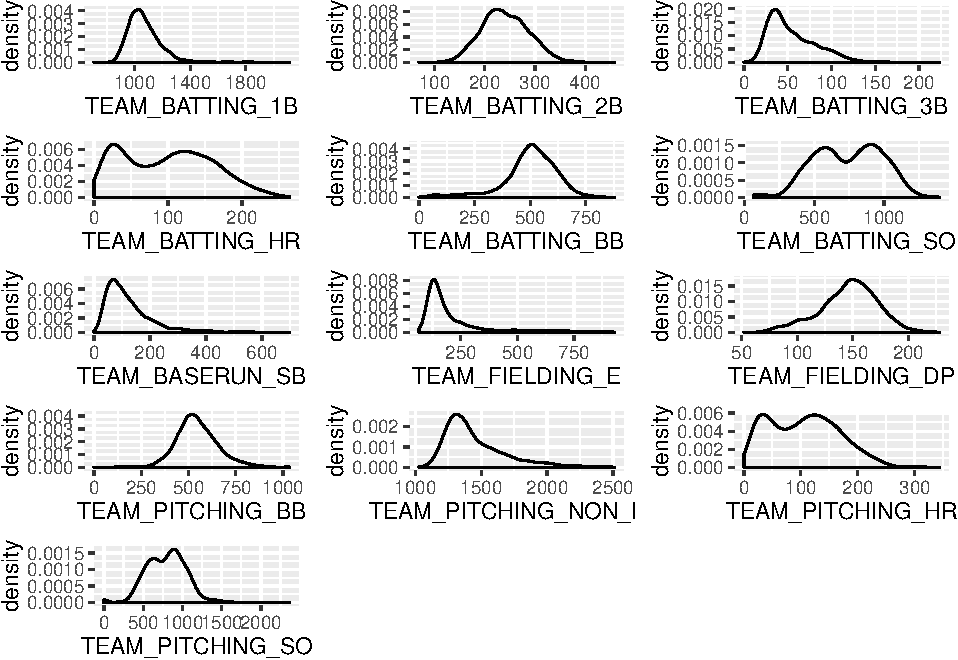
\includegraphics{DATA621-Homework-1_files/figure-latex/unnamed-chunk-17-1.pdf}

\section{Build Models}\label{build-models}

\subsection{Model 1: Backwards Selection - NAs in
dataset}\label{model-1-backwards-selection---nas-in-dataset}

For our first model, we used backward selection. In this method we
calculate the linear model starting with all predictor variables, then
remove the value with the highest P value until we have no signficance
values greater than 0.05.

The model that results from backward selection on complete data only is:

\[Team Wins = 60.5 - 0.031singles - 0.080doubles + 0.152triples + 0.129homeruns + 0.151strikeouts.batting + \]\\
\[ 0.070stolen.bases + 0.057pitching-non-homeruns - 0.111pitching.walks - \]\\
\[ 0.022pitching.strikeouts - 0.119errors - 0.113double.plays\]

Several of these coefficients indicate a relationship with wins that
does not make sense. For instance, the coefficients for single and
doubles are both negative. Strikeouts while batting is positive. We
decided to keep this model despite these results because, while it may
be assumed that more singles and doubles should indicate a better team
and more wins, it also says something about the pitching they faced. It
may be that the model is influenced by seasons where weak pitching
resulted in many hits that didn't correspond to more wins - just higher
scoring games. Without the ability to adjust these metrics by `at bats'
(which is used for batter averages) we cannot improve on this aspect of
the model.

\begin{verbatim}
## Warning in model.matrix.default(mt, mf, contrasts): the response appeared
## on the right-hand side and was dropped
\end{verbatim}

\begin{verbatim}
## Warning in model.matrix.default(mt, mf, contrasts): problem with term 1 in
## model.matrix: no columns are assigned
\end{verbatim}

\begin{verbatim}
## 
## Call:
## lm(formula = TARGET_WINS ~ TARGET_WINS + TEAM_BATTING_1B + TEAM_BATTING_2B + 
##     TEAM_BATTING_3B + TEAM_BATTING_HR + TEAM_BATTING_BB + TEAM_BASERUN_SB + 
##     TEAM_PITCHING_NON_HR + TEAM_PITCHING_BB + TEAM_PITCHING_SO + 
##     TEAM_FIELDING_E + TEAM_FIELDING_DP, data = train)
## 
## Residuals:
##     Min      1Q  Median      3Q     Max 
## -32.121  -7.181   0.137   6.900  29.800 
## 
## Coefficients:
##                       Estimate Std. Error t value Pr(>|t|)    
## (Intercept)          60.493336   5.982599  10.112  < 2e-16 ***
## TEAM_BATTING_1B      -0.031955   0.014924  -2.141   0.0324 *  
## TEAM_BATTING_2B      -0.080514   0.015485  -5.199 2.22e-07 ***
## TEAM_BATTING_3B       0.152310   0.022157   6.874 8.55e-12 ***
## TEAM_BATTING_HR       0.128822   0.007967  16.169  < 2e-16 ***
## TEAM_BATTING_BB       0.150695   0.035443   4.252 2.23e-05 ***
## TEAM_BASERUN_SB       0.070017   0.005508  12.713  < 2e-16 ***
## TEAM_PITCHING_NON_HR  0.057361   0.013417   4.275 2.01e-05 ***
## TEAM_PITCHING_BB     -0.111511   0.033533  -3.325   0.0009 ***
## TEAM_PITCHING_SO     -0.022159   0.002169 -10.217  < 2e-16 ***
## TEAM_FIELDING_E      -0.119393   0.007140 -16.722  < 2e-16 ***
## TEAM_FIELDING_DP     -0.112805   0.012255  -9.205  < 2e-16 ***
## ---
## Signif. codes:  0 '***' 0.001 '**' 0.01 '*' 0.05 '.' 0.1 ' ' 1
## 
## Residual standard error: 10.17 on 1822 degrees of freedom
##   (442 observations deleted due to missingness)
## Multiple R-squared:  0.4055, Adjusted R-squared:  0.4019 
## F-statistic:   113 on 11 and 1822 DF,  p-value: < 2.2e-16
\end{verbatim}

Residual plots from Model 1 indicate a random distribution of residuals,
with some deviations at extreme values.\\
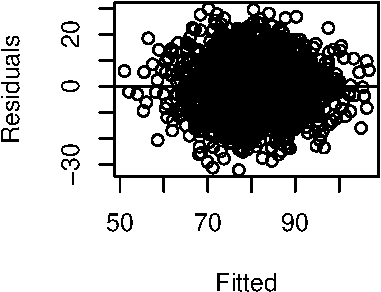
\includegraphics{DATA621-Homework-1_files/figure-latex/unnamed-chunk-21-1.pdf}
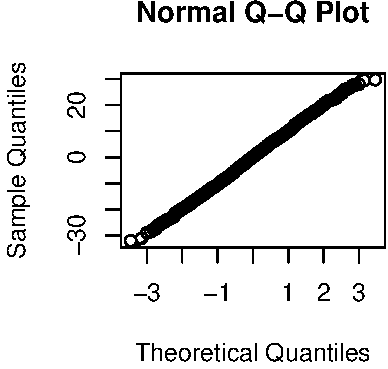
\includegraphics{DATA621-Homework-1_files/figure-latex/unnamed-chunk-21-2.pdf}

\subsection{Model 1: Backwards Selection - Using imputed values dataset
(no
NAs)}\label{model-1-backwards-selection---using-imputed-values-dataset-no-nas}

When using the dataset with imputed NA values, all variables are
signficant.

\begin{verbatim}
## 
## Call:
## lm(formula = TARGET_WINS ~ ., data = train.fill.nas)
## 
## Residuals:
##     Min      1Q  Median      3Q     Max 
## -62.296  -8.471   0.229   8.688  54.657 
## 
## Coefficients:
##                        Estimate Std. Error t value Pr(>|t|)    
## (Intercept)           1.089e+01  5.399e+00   2.017  0.04378 *  
## TEAM_BATTING_1B       4.134e-02  3.702e-03  11.167  < 2e-16 ***
## TEAM_BATTING_2B       3.171e-02  7.584e-03   4.181 3.01e-05 ***
## TEAM_BATTING_3B       1.064e-01  1.704e-02   6.242 5.13e-10 ***
## TEAM_BATTING_HR       8.188e-02  2.961e-02   2.765  0.00573 ** 
## TEAM_BATTING_BB       4.964e-02  6.209e-03   7.994 2.06e-15 ***
## TEAM_BATTING_SO       2.325e-05  2.630e-03   0.009  0.99295    
## TEAM_BASERUN_SB       2.190e-02  4.256e-03   5.146 2.89e-07 ***
## TEAM_BASERUN_CS       4.432e-03  1.284e-02   0.345  0.73005    
## TEAM_PITCHING_NON_HR  3.200e-03  1.889e-03   1.694  0.09034 .  
## TEAM_PITCHING_HR      2.243e-02  2.652e-02   0.846  0.39771    
## TEAM_PITCHING_BB     -2.585e-02  5.793e-03  -4.463 8.48e-06 ***
## TEAM_PITCHING_SO     -7.938e-04  2.086e-03  -0.381  0.70359    
## TEAM_FIELDING_E      -4.463e-03  2.951e-03  -1.512  0.13057    
## TEAM_FIELDING_DP     -1.050e-01  1.245e-02  -8.436  < 2e-16 ***
## ---
## Signif. codes:  0 '***' 0.001 '**' 0.01 '*' 0.05 '.' 0.1 ' ' 1
## 
## Residual standard error: 13.37 on 2261 degrees of freedom
## Multiple R-squared:  0.2839, Adjusted R-squared:  0.2795 
## F-statistic: 64.02 on 14 and 2261 DF,  p-value: < 2.2e-16
\end{verbatim}

\subsection{Model 2:}\label{model-2}

For this model, we take advantage of principal component analysis
method. First, we used an orthogonal transformation to convert our
variables into a set of values of linearly uncorrelated variables, which
called principal components. And then we chose the first five principal
components that account for around 95\% proportion of variance in the
data. Finally, we used those chosen principal components to build a
linear regression model.

\begin{Shaded}
\begin{Highlighting}[]
\CommentTok{# PCA analysis}
\NormalTok{Predictor <-}\StringTok{ }\NormalTok{train.fill.nas$TARGET_WINS}
\NormalTok{A <-}\StringTok{ }\KeywordTok{as.matrix}\NormalTok{(}\KeywordTok{select}\NormalTok{(train.fill.nas,-TARGET_WINS))}
\NormalTok{pca <-}\StringTok{ }\KeywordTok{princomp}\NormalTok{(A,}\DataTypeTok{center=}\NormalTok{T,}\DataTypeTok{scale.=}\NormalTok{T)}
\KeywordTok{plot}\NormalTok{(pca)}
\end{Highlighting}
\end{Shaded}

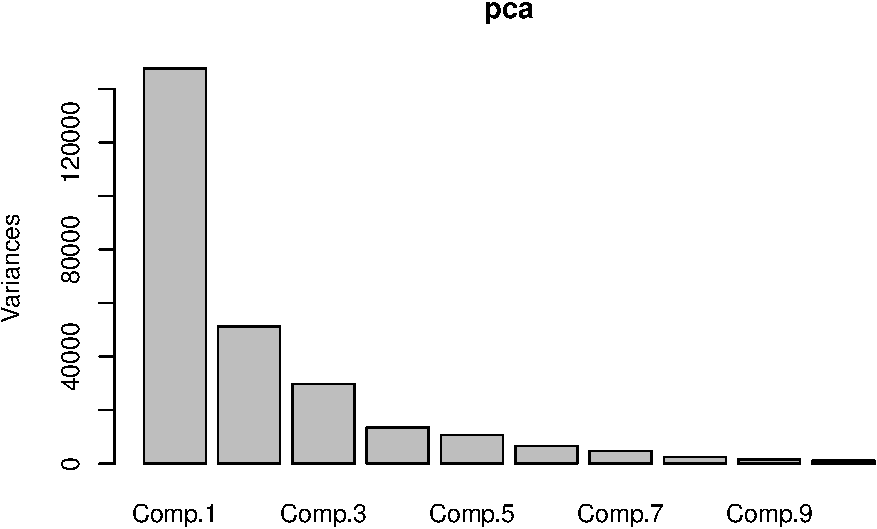
\includegraphics{DATA621-Homework-1_files/figure-latex/unnamed-chunk-23-1.pdf}

\begin{Shaded}
\begin{Highlighting}[]
\KeywordTok{summary}\NormalTok{(pca)}
\end{Highlighting}
\end{Shaded}

\begin{verbatim}
## Importance of components:
##                             Comp.1      Comp.2      Comp.3       Comp.4
## Standard deviation     384.2192847 226.6345455 172.6607355 116.27354942
## Proportion of Variance   0.5445055   0.1894507   0.1099591   0.04986614
## Cumulative Proportion    0.5445055   0.7339561   0.8439152   0.89378138
##                              Comp.5      Comp.6     Comp.7       Comp.8
## Standard deviation     103.71302363 81.83448302 68.5373215 50.860622880
## Proportion of Variance   0.03967441  0.02470112  0.0173260  0.009541294
## Cumulative Proportion    0.93345579  0.95815691  0.9754829  0.985024199
##                              Comp.9      Comp.10      Comp.11      Comp.12
## Standard deviation     39.933740233 34.121932816 22.431916142 21.654141916
## Proportion of Variance  0.005881985  0.004294486  0.001855994  0.001729521
## Cumulative Proportion   0.990906184  0.995200670  0.997056664  0.998786186
##                             Comp.13      Comp.14
## Standard deviation     16.711557594 7.0575516547
## Proportion of Variance  0.001030096 0.0001837182
## Cumulative Proportion   0.999816282 1.0000000000
\end{verbatim}

\begin{Shaded}
\begin{Highlighting}[]
\NormalTok{pca <-}\StringTok{ }\KeywordTok{as.data.frame}\NormalTok{(pca$scores[,}\DecValTok{1}\NormalTok{:}\DecValTok{5}\NormalTok{])}
\NormalTok{train_pca <-}\StringTok{ }\KeywordTok{cbind}\NormalTok{(}\DataTypeTok{TARGET_WINS=}\NormalTok{Predictor,pca)}
\KeywordTok{head}\NormalTok{(train_pca)}
\end{Highlighting}
\end{Shaded}

\begin{verbatim}
##   TARGET_WINS    Comp.1      Comp.2     Comp.3     Comp.4     Comp.5
## 1          39 -98.71852 -139.043689   31.45711 -46.864102 97.1932047
## 2          70 583.58046   -2.050978  102.90234 153.928657 27.2148864
## 3          86 329.56343  -77.523496   39.83319  75.376295  9.8793404
## 4          70 266.43069  -35.978839 -129.80400 -63.649910 -0.7413798
## 5          82 334.73175 -120.281629 -129.60476  -3.396324 -1.7657030
## 6          75 397.45965  -82.204331 -170.81421 -12.825813 25.8195895
\end{verbatim}

\begin{Shaded}
\begin{Highlighting}[]
\CommentTok{# Separate data into two parts, one for training models and the other for testing models}
\KeywordTok{set.seed}\NormalTok{(}\DecValTok{45}\NormalTok{)}
\NormalTok{inTrain_pca <-}\StringTok{ }\KeywordTok{createDataPartition}\NormalTok{(}\DataTypeTok{y=}\NormalTok{train_pca$TARGET_WINS, }\DataTypeTok{p=}\FloatTok{0.7}\NormalTok{,}\DataTypeTok{list=}\OtherTok{FALSE}\NormalTok{)}
\NormalTok{training_pca <-}\StringTok{ }\NormalTok{train_pca[inTrain_pca,]}
\NormalTok{testing_pca <-}\StringTok{ }\NormalTok{train_pca[-inTrain_pca,]}

\CommentTok{# Build a model}
\NormalTok{lm2_a <-}\StringTok{ }\KeywordTok{lm}\NormalTok{(TARGET_WINS ~}\StringTok{ }\NormalTok{., }\DataTypeTok{data=}\NormalTok{training_pca)}
\KeywordTok{summary}\NormalTok{(lm2_a)}
\end{Highlighting}
\end{Shaded}

\begin{verbatim}
## 
## Call:
## lm(formula = TARGET_WINS ~ ., data = training_pca)
## 
## Residuals:
##     Min      1Q  Median      3Q     Max 
## -55.671  -9.384   0.770   9.790  63.983 
## 
## Coefficients:
##               Estimate Std. Error t value Pr(>|t|)    
## (Intercept) 80.8683822  0.3732178 216.679  < 2e-16 ***
## Comp.1      -0.0043681  0.0009728  -4.490 7.62e-06 ***
## Comp.2       0.0022652  0.0016569   1.367  0.17178    
## Comp.3       0.0242682  0.0021596  11.237  < 2e-16 ***
## Comp.4      -0.0086712  0.0032026  -2.708  0.00685 ** 
## Comp.5       0.0003899  0.0036242   0.108  0.91433    
## ---
## Signif. codes:  0 '***' 0.001 '**' 0.01 '*' 0.05 '.' 0.1 ' ' 1
## 
## Residual standard error: 14.9 on 1589 degrees of freedom
## Multiple R-squared:  0.08909,    Adjusted R-squared:  0.08622 
## F-statistic: 31.08 on 5 and 1589 DF,  p-value: < 2.2e-16
\end{verbatim}

\subsection{Model 3: Using Variable
Ratios}\label{model-3-using-variable-ratios}

As discussed above, several variables display collinearity. Some
variables by definition have the same sum (for every one batting walk,
another team has a pitching walk) and some variables indicate a hidden
variable (stolen bases and caught stealing appear to indicate stolen
base attempts). Therefore, we used several ratios among predictor
variables.

\subsection{Deriving Ratio Variables}\label{deriving-ratio-variables}

One area of interest was whether or not variables relative to another
relevant variable would prove to be a better predictor than the raw data
on its own. To test this out, we created 3 ratio variables: Stolen base
percentage, HR to Strikout (batting) percentage, and Strikeout to Walk
(pitching, otherwise known as K/BB) percentage. These ratios were
calculated from the dataset that ignored records with missing values
(discussed later).

Stolen base percentage measured stolen bases over stolen bases plus
caught stealing, which would constitue total stolen base attempts.
Plotting the graphs of stolen bases against wins and comparing to stolen
base percentage against wins showed that the percentage had a slightly
positive linear relationship with wins. Stolen bases did have a positive
correlation with wins (.1203), but the percentage had a stronger
relationship (.172). Due to the stronger and more linear relationship,
we will use the percentage over stolen bases.

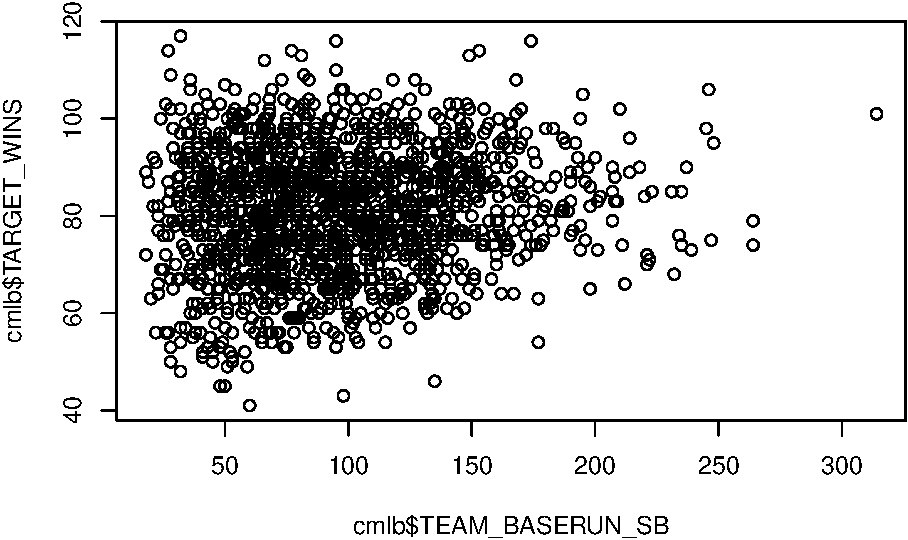
\includegraphics{DATA621-Homework-1_files/figure-latex/unnamed-chunk-24-1.pdf}
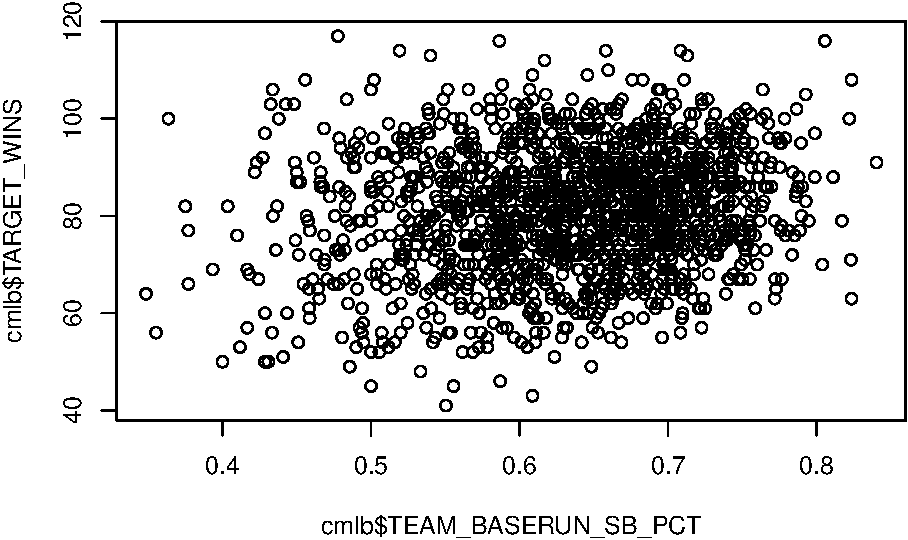
\includegraphics{DATA621-Homework-1_files/figure-latex/unnamed-chunk-24-2.pdf}

HR to Strikout percentage was derived because batting HRs and Strikeouts
had a correlation of .6402. Thus perhaps more valuable than knowing the
gross amounts of either variable would be the ratio of one to the other.
And it did appear graphically that there was a stronger linear
relationship using the HR to Strikout ratio than simply HRs. The homerun
to strikeout percentage was more highly correlated with wins (.419) than
homeruns (.2834), so we will use Home Run to Strikeout percenatage in
our model.

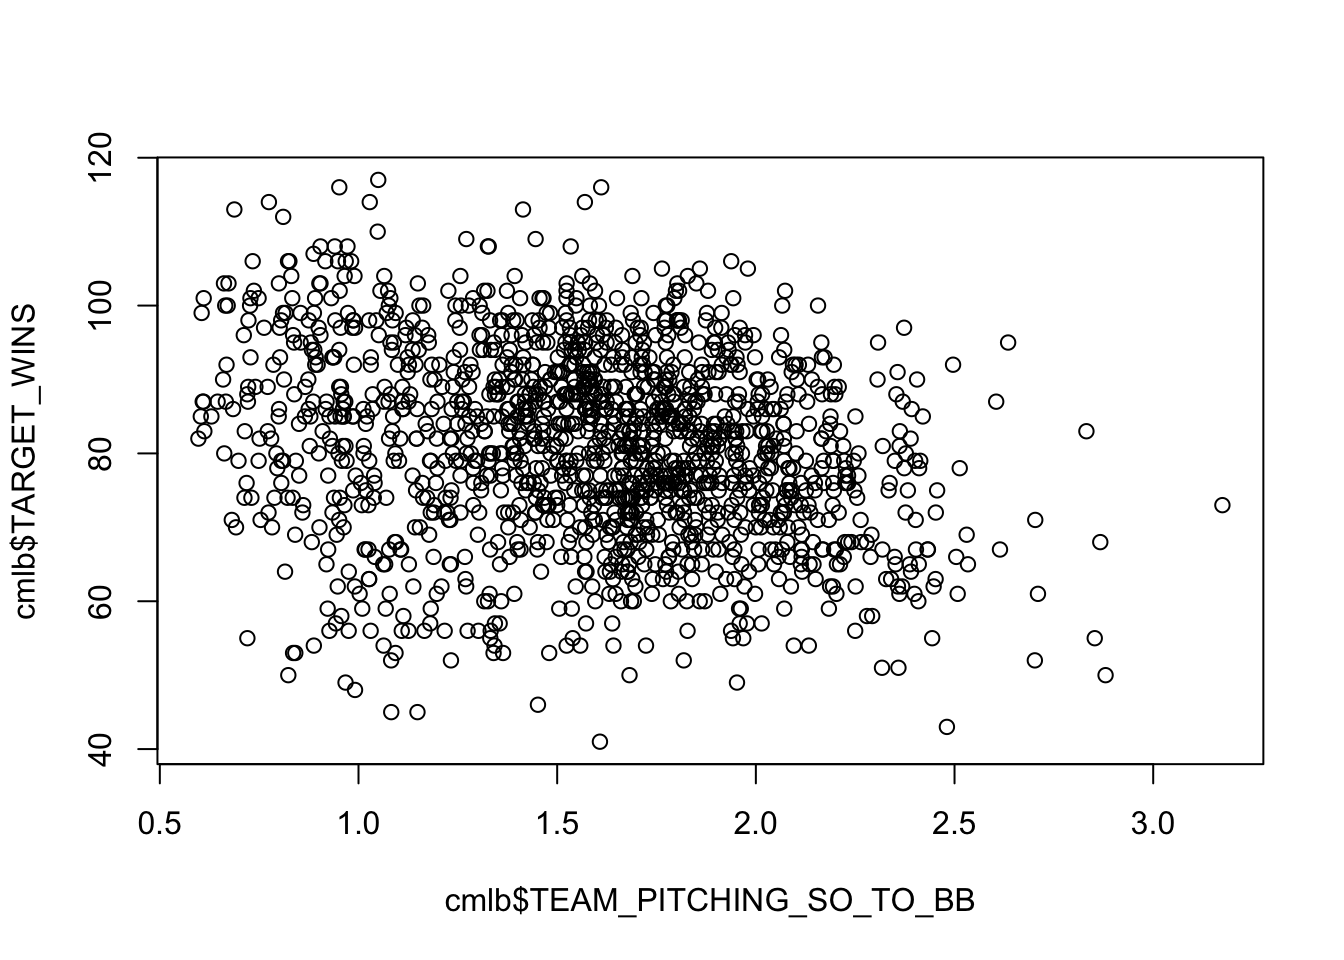
\includegraphics{DATA621-Homework-1_files/figure-latex/unnamed-chunk-25-1.pdf}
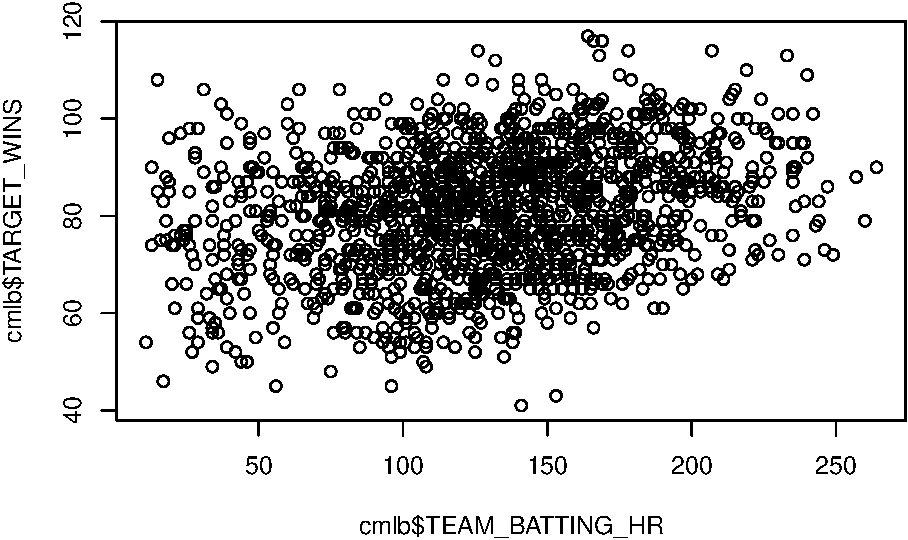
\includegraphics{DATA621-Homework-1_files/figure-latex/unnamed-chunk-25-2.pdf}

For pitching, Strikeout to Walk (K/BB) Ratio was calculated.
\href{http://www.beyondtheboxscore.com/2012/11/25/3686732/stop-using-k-bb}{This
is a traditional baseball statistic that has currently come under
scrutiny with the modernization of baseball analysis.} With that in mind
we thought it would be of interest to see what kind of impact including
this variable would have on a model.

Counterintuitively, both Strikouts and K/BB showed negative correlations
with wins (-.067 and -0.2312). Since strikouts are generally a good
thing for the pitching team, and walks are generally bad, this is a
surprising finding. One would think that maximizing the ratio of good
events to bad events would ultimately lead to more wins, but this
decidedly not the case. Further investigation into this matter would be
of interest, but is beyond both the scope and the available data in this
study.

K/BB appeared to have a slightly more linear relationship visually, so
this combined with it's higher correlation made in the factor that we
chose for the ratio model.\\
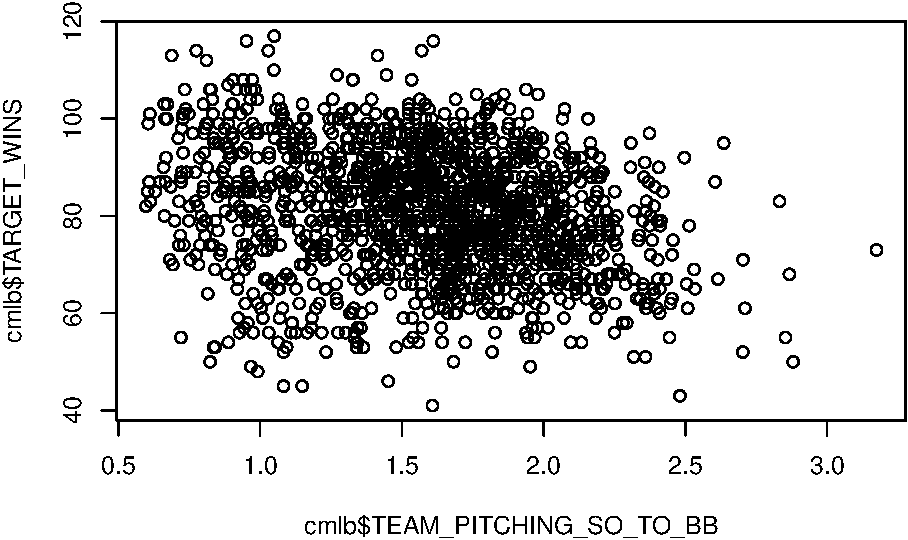
\includegraphics{DATA621-Homework-1_files/figure-latex/unnamed-chunk-26-1.pdf}
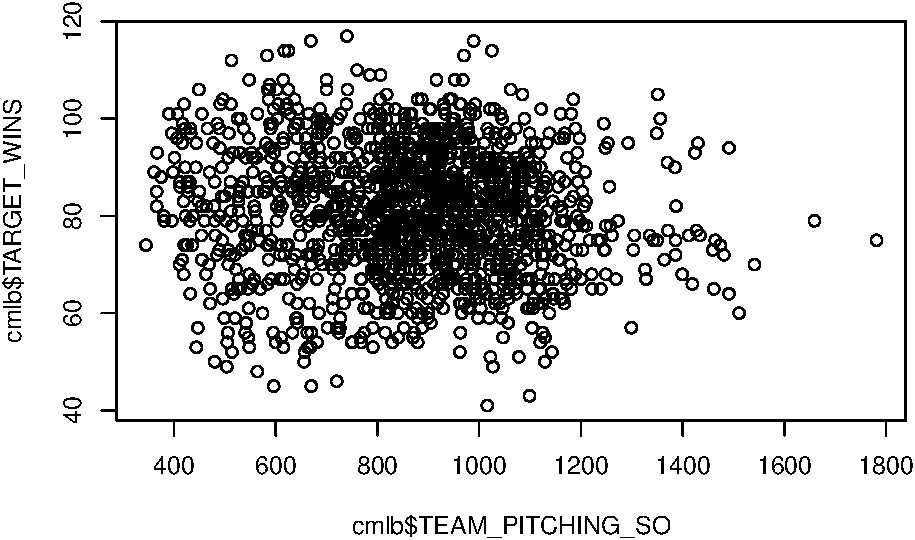
\includegraphics{DATA621-Homework-1_files/figure-latex/unnamed-chunk-26-2.pdf}

In the end, the ratio model wound up being calculated as follows:

Predicted\_wins = 56.44 + 34.16(StolenBasePct) + 96.45(HR/SO) -
7.5(K/BB)

\section{Select Model: Evaluating The
Models}\label{select-model-evaluating-the-models}

The below table shows the 3 models and their corresponding statistics
for selecting an appropriate model:

\begin{longtable}[c]{@{}llll@{}}
\toprule
Model Name & Mean Sq. Error & R Squared & F Stat\tabularnewline
\midrule
\endhead
lm1\_a & 102.812661984364 & 0.40552401333798 &
78.1113972466726\tabularnewline
lm1\_b & 177.610315532526 & 0.283890840739642 &
149.265969291314\tabularnewline
ratio\_model & 120.359246926108 & 0.252517590606597 &
58.9419811545502\tabularnewline
pca & 221.140824912914 & 0.0890865092903272 &
20.3792678947301\tabularnewline
\bottomrule
\end{longtable}

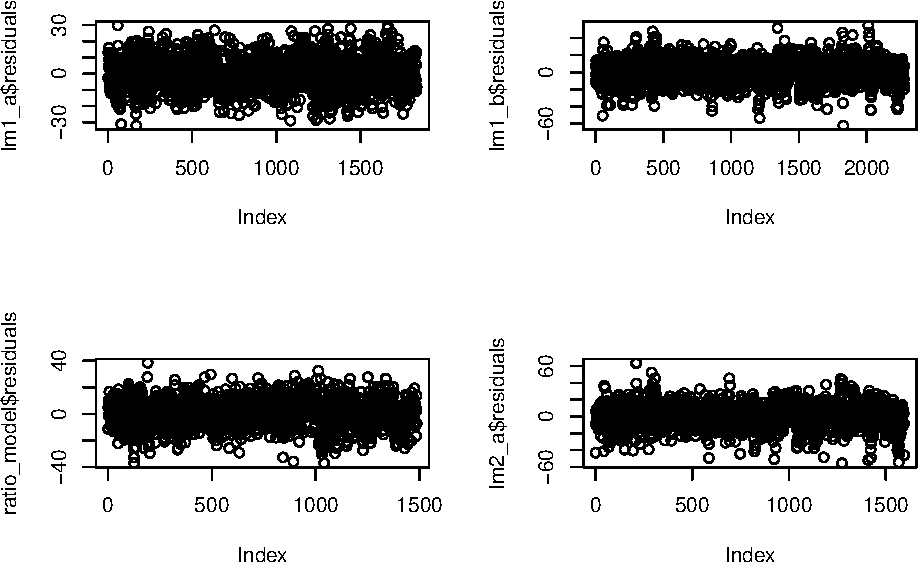
\includegraphics{DATA621-Homework-1_files/figure-latex/unnamed-chunk-27-1.pdf}

\subsubsection{Predicted wins}\label{predicted-wins}

The first model fit, lm1\_a, used backwards stepwise selection and the
dataset containing NAs. It has the lowest mean square error, highest
coefficient of determination and second highest F-Statistic. It's
residuals do not indicate any red flags. Therefore, we have chosen it as
our best model for predicting team wins.

Using the predict.lm() function, we use the first linear model created,
lm1\_a, to predict team wins from the evaluation dataset. This density
plot of the wins output resembles the training data plot above. This is
a good indication our model is reasonable.

\begin{verbatim}
## Warning: Removed 54 rows containing non-finite values (stat_density).
\end{verbatim}

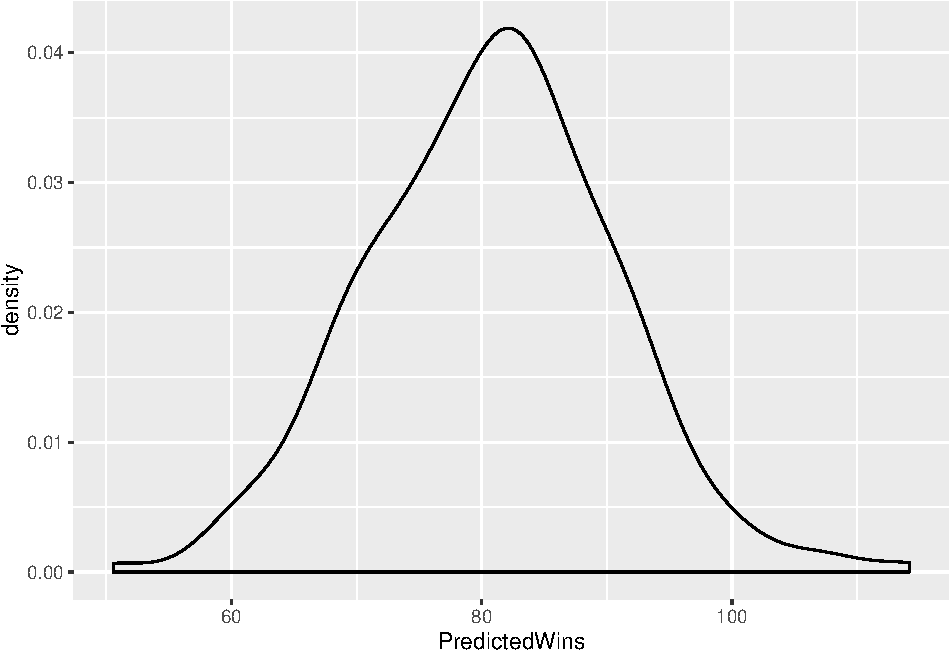
\includegraphics{DATA621-Homework-1_files/figure-latex/unnamed-chunk-29-1.pdf}

\begin{Shaded}
\begin{Highlighting}[]
\KeywordTok{write.csv}\NormalTok{(predicted.wins, }\DataTypeTok{file =} \StringTok{"model_predicted_wins.csv"}\NormalTok{)}
\end{Highlighting}
\end{Shaded}

\end{document}
